\section{中國政府錯解香港歷史了嗎?}

中國政府對香港歷史的描述和歷史上中國大陸對香港的各種描述一樣,往往是為訴說者的立場服務。不同時期的中國政府更會按其當時的形勢改變官方的香港描述,就算弄得前後矛盾也在所不惜,以達所需的政治效果。

把時間軸拉到上世紀九十年代,香港主權移交前的一段時間。這時期中國大陸前所未有地出現大量關於香港的官方宣傳,無論是文字的或是影像的都數之不盡。表面上,這些官方宣傳是要向中國大陸民眾介紹香港的各方面,但和任何的官方宣傳一樣,背後也有其隱含的政治立場,以下以學者王宏志就紀錄片《香港滄桑》的分析為例。

\begin{figure}[htbp]
    \centering
    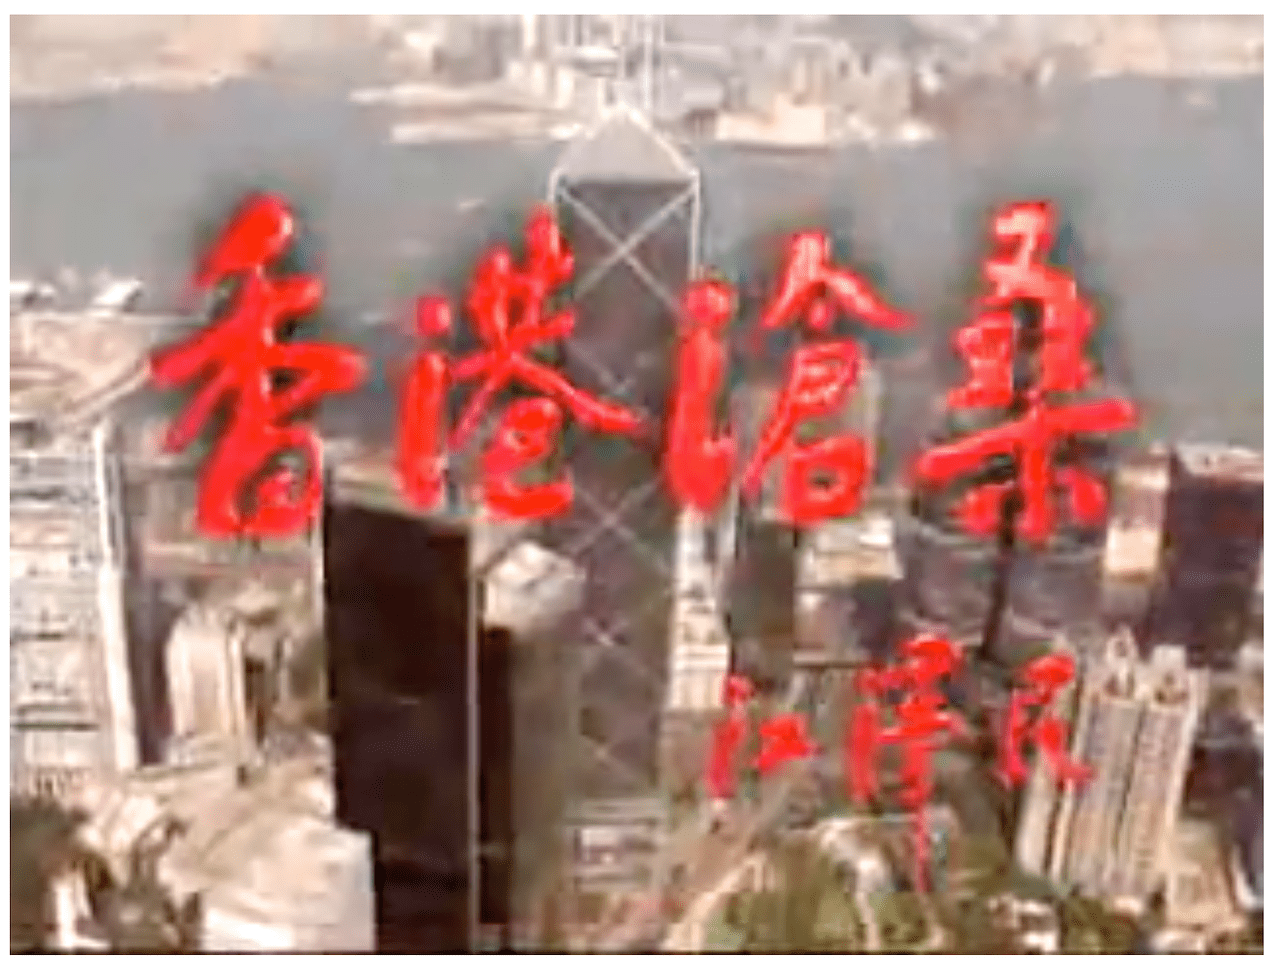
\includegraphics[width=0.7\textwidth]{c02/hkdocumentary.png}
    \caption{《香港滄桑》片頭畫面} 
\end{figure}

《香港滄桑》是由中央電視台製作的紀錄片,於一九九六年七月一日,也就是主權移交日之前一年首播,合共十二集,這兒集中談序章開首十數分鐘的內容。這段片段首先強調香港從古代開始與中國大陸的連結,如考古文物推斷的文化交流。說到英殖時期開始,則強調香港人在英治下所受的不公平對待和反抗,並以海員大罷工和省港大罷工為例。至於英治對香港的正面影響則避重就輕,和康有為與孫中山採取的角度相反。這段內容和中國大陸同期的史學著作十分相似,可謂典形的愛國主義的史學,以中國本位來訴說香港歷史,如強調香港問題源於帝國主義對中國的侵略,香港人民的利益向中國大陸人民的利益根本一致,而香港的反帝運動也是中國的反帝民族覺醒的一部分。

這些描述當然十分之有選擇性,不過要說到最明顯的政治處理,就要說到上世紀二次大戰結束的一段。解說詞這樣說:

\begin{displayquote}
    「全中國人民包括香港同胞無不熱切盼望香港早日回到祖國的懷抱,國民黨政府曾經想以戰勝國的身分從日本佔領軍手中收回香港,後因為蔣介石急於打內戰,向頑固堅持殖民立場的英國政府妥協,香港問題的解決終成泡影(……)中國人只能眼巴巴的看著英國人又一次大踏步的回到了香港,英國的國旗再一次插在這塊中國人的土地上。」(《香港滄桑》)
\end{displayquote}

這段描述本身的問題,已有很多歷史學者談過。例如說當時的香港的香港人希望回到中國,是明顯與事實不乎。恰恰相反的,是香港作為殖民地的地位,吸收了二戰結束後過百萬害怕中國內戰的難民前來香港。至於說「蔣介石急於打內戰」而放棄香港,也是明顯扭曲歷史。

但更值得關心的問題,是即使假設這段解說完全成立,仍會產生嚴重的內在矛盾,無法自圓其說。在說罷二次大戰之後,片段就轉為介紹中共在國共內戰中得勝,解放軍來到香港邊界的深圳河,解說詞表明當時的解放軍絕對有能力從英軍手上奪取香港,只是基於中國整體的戰略部署而沒有這樣做,也就是所謂的「長期打算,充分利用」。

這說法對關心香港歷史的讀者來說,大多耳熟能詳。但將之和先前緊接有關二次大戰的解說放在一起,就明顯地突兀了。片段首先聲稱香港人在英治之下受苦,希望回到中國;片段繼而對於國民政府沒有收回香港,表示責難;然而到了中共的時候,卻聲稱中共有能力收回香港,卻選擇不收回。把這三點放在一起,則必然產生三個難以解答的問題:首先,如果國民政府沒有收回香港是應該被責難的,那麼中共有能力卻不收回香港,是否更應該被責難呢?再者,中共聲稱為了整體的戰略部署而不收回香港,是否代表了香港人在英治之下所受的痛苦在中共眼中是次要的,只要有被利用的價值就不用計較,即是說港人的幸福在這段時間是為了全國整體的戰略部署而被犧牲?如是者,全國上下在歷史上對香港豈非有所虧欠?

這些明顯的自相矛盾能夠被完全忽視,因為紀錄片的目的恰好也是要「充分利用」一九九七帶來的機會,而香港同樣是被利用的一方。紀錄片雖然以香港為題,但香港並不是主角。借用近年流行的說法,「中華民族的偉大復興」才是主角,香港只是這個主題的其中一頁,用來指出中國在共產黨的領導下終於「洗脫」了晚清以來受帝國主義壓迫的「百年屈辱」。因此,香港歷史當中與此主題相關的就會被大書特書,相反的就被隱去不提。

如是者,既然要以中國為本位的立場來談論香港的歷史,如果香港人有任何反抗英治的行動,也要視之為中國民族革命的一部份來描述。這種愛國主義史學當然是偏頗的,最起碼沒有以地方人民的權益為解釋歷史的首要考慮。而這偏頗也會妨礙客觀分析英治香港的實際情況,例如華人社會內部以及統治者和被統治者之間的複雜關係。前面提到海員大罷工和省港大罷工,有歷史學者就提出在港華商於過程中也有自己的利益盤算。又有文化研究學者以「勾結式殖民主義」來解釋香港殖民統治中華人頭領在中英間調節迥轉以至多重效忠的特質,也和愛國主義史學的說法相去甚遠。當時的華商不止積極協助港英政府終止省港大罷工等的紛爭,更不時捐款支持英國一些與香港無關的重大事件,從愛爾蘭饑荒到南非波耳戰爭不等。

說到底,愛國主義史觀由於把國家作為唯一的分析單位,會錯過超越國家的力量,以及國家之內的差異。當然,這很可能就是愛國主義史觀推動者的目的:當眼前的所有問題都是境外勢力做成的,那麼境內既得利益者過去和現在犯過的錯誤,或社會現存的制度和結構性問題,都可被隱藏起來。

中國大陸對香港歷史的官方描述常有自相矛盾之處,類似的例子還有不少。不少中國大陸出版的香港歷史書都會反覆強調中國政府早就宣佈不受有關香港的三個中英條約的約束,有權決定在何時收回香港;與此同時,卻又會反覆提出中英《展拓香港界址專條》將於一九九七年六月三十日到期,英國是基於條約的壓力才與中國展開談判,更常使用「九七大限」的字眼來說明英方於談判中的劣勢。這些歷史書說到七十年代香港前途未明時,會把信心危機和移民潮視為對英方的壓力,儘管這些描述恰恰說明「香港同胞熱切期待回歸祖國」的說法不乎事實。

說到中國大陸對香港主權移交的選擇性描述,最有選擇性的地方莫過於《中英聯合聲明》的簽署儀式。作為「香港回歸祖國」的基礎,這個儀式本來是應該被珍而重之並大書特書的。然而這儀式在中國大陸的官方描述中出現得不多。如果是圖片的話,通常使用一張覆蓋整個會場的廣角鏡頭照片,差不多無法看清楚人臉,更別說他們在做什麼。無論是位於北京天安門旁的國家博物館,還是香港自己的歷史博物館,用的也是這一張照片。如果是影片的話,則會避過雙方簽字的一刻,而用上之後時任英國首相的戴卓爾夫人和時任中國中央軍委主席的鄧小平祝酒的片段。在此安排下,代表中方簽署的官員是誰,就難以在這些描述中找到。其實當時代表中方簽署《中英聯合聲明》的是時任中國國務院總理的趙紫陽;然而由於趙紫陽於八九民運後被迫下台,儘管他在這歷史時刻有至關重要的角色,來到今天就被略去不提了。

\begin{figure}[htbp]
    \centering
    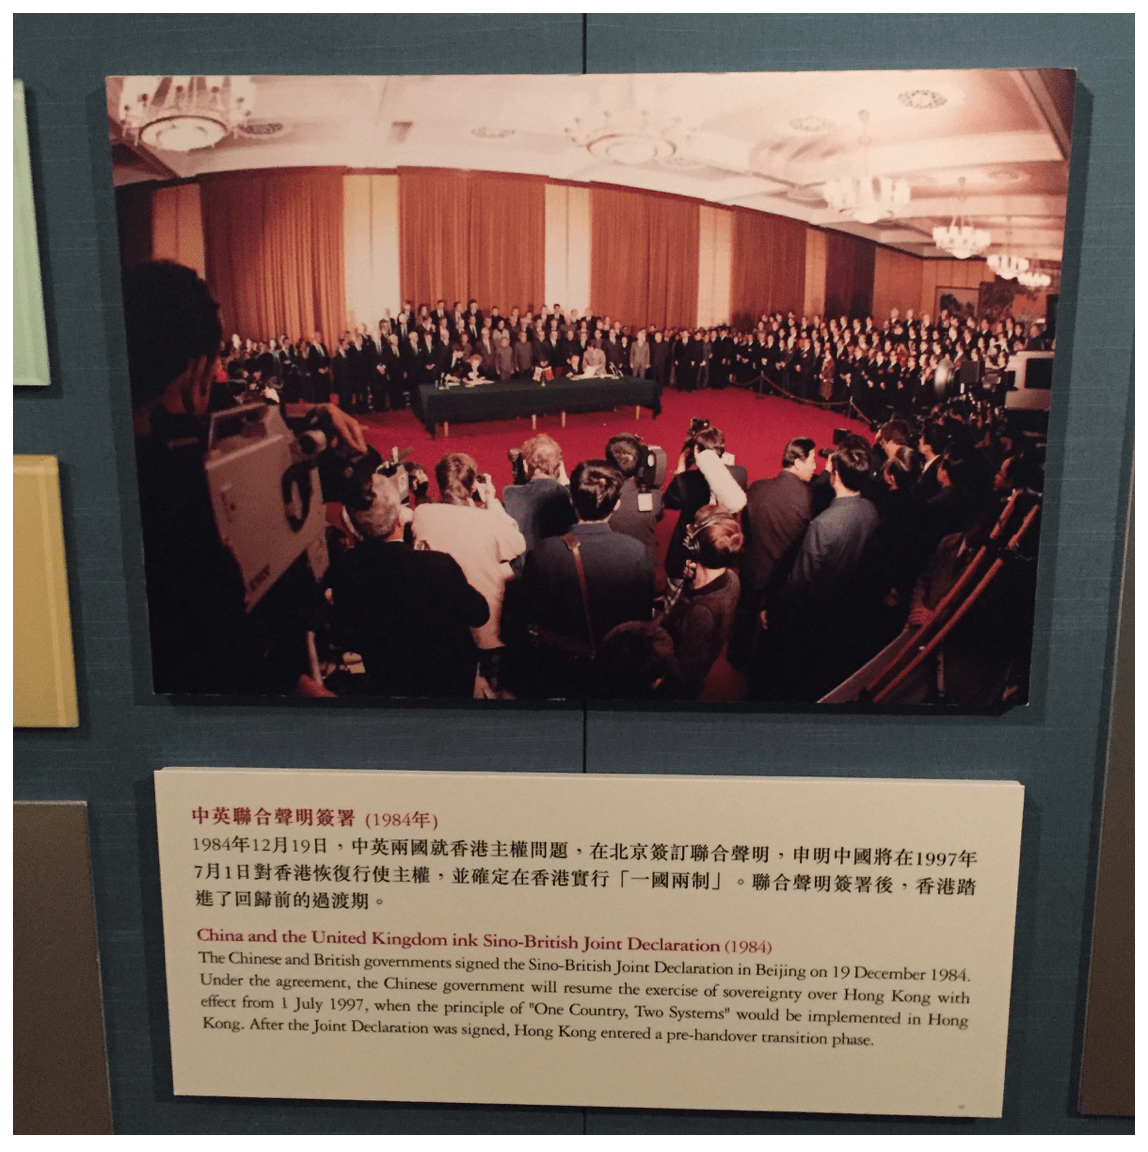
\includegraphics[width=0.7\textwidth]{c02/h-kmuseum-jointdeclaration.png}
    \caption{香港歷史博物館中介紹中英聯合聲明簽署的圖片} 
\end{figure}

中國大陸官方的選擇性歷史詮釋,當然不僅限於香港。無論是把平凡甚至不存在的事件英雄化或把違反人性的暴行抹去不提的案例均俯拾皆是(長春圍城戰就是一例)。反過來說,對香港歷史的選擇性詮釋,也不止於中國大陸官方。英國官方對香港歷史的描述往往會以「荒島」(Barren Rock)作為開端,暗示香港開埠以來的成功都是英國人帶來的。實情是在英國人來到之前香港一帶已有不少人居住;陸上有農民,海上有漁民、商旅,以至海盗等等,「荒島」一說是誇張了。

選擇性歷史詮釋的問題,在於會把偏見強化,只看到和自己期望一致的事情,有違既有立場的事例則當作看不見或視為虛假。長此下去,認識就會變得和真實越走越遠,甚至連自己也被欺騙。這問題值得討論,是因為當基於主觀偏見的行為和客觀事實有所衝突,其落差無論對己對人都可帶來很大威脅。在香港,這些有選擇性的描述在香港特區成立早期帶來的問題不算明顯,到了後來中國政府對香港政治和社會的干預越來越多的時候,片面理解所帶來政策不當和引發的衝突就變得激烈了。

\rule[-10pt]{15cm}{0.05em}

伸延閱讀:

王宏志(2000):《歷史的沉重:從香港看中國大陸的香港史論述》,香港:牛津大學出版社。

張少強(2011):〈香港:地緣政治與香港研究〉,呂大樂等編《香港.生活.文化》,香港:牛津大學出版社。

蔡榮芳(2001):《香港人之香港史1841-1945》,香港:牛津大學出版社。

羅永生(2015):《勾結共謀的殖民權力》,香港:牛津大學出版社。